O modelo foi implementado em linguagem de programação Python (versão 2.7.13), que é uma linguagem livre, de fácil entendimento [6] e que vem sendo utilizada e difundida pela comunidade científica de Neurociência Computacional [7]. Os elementos neuronais foram implementados utilizando as bibliotecas do simulador NEURON [8] para a linguagem Python. A rede de MNs foi implementada utilizando o NetPyNE [9].

O modelo neuromuscular desenvolvido é composto por apenas três MNs (modelo simplificado) e as fibras musculares por eles inervadas. As fibras musculares pertencentes a uma determinada unidade motora são referidas como unidades musculares (UMs). Os modelos individuais dos MNs e das UMs serão descritos abaixo.

\paragraph{Modelo de MN alpha}
Foram representados modelos de MNs dos tipos S (\emph{slow}, que inerva fibras musculares lentas e resistentes à fadiga), FR (\emph{fast fatigue resistant}, fibras rápidas e resistentes à fadiga) e FF (\emph{fast fatigable}, fibras rápidas e fatigáveis). Estes modelos foram baseados na proposta de Cisi e Kohn [5], em que a morfologia dos MNs é sintetizada em dois compartimentos acoplados por uma condutância. Um compartimento representa a árvore dendrítica, que neste estudo foi suposta passiva, e o outro compartimento representa o corpo celular (ou soma). O circuito elétrico equivalente dos modelos está ilustrado na Figura 1. As condutâncias ativas somáticas são responsáveis pelo decurso temporal do PA e da AHP (\emph{after hyperpolarization}). Estas condutâncias (Na+, K+, persistente de Na+ e lenta de K+) foram parametrizadas e validadas em um estudo anterior do nosso laboratório [10]. Os parâmetros geométricos e eletrotônicos (Tabela 1) foram baseados em estudos experimentais anteriores com MNs de gatos anestesiados [11-13].

\begin{figure}[h]
  \centering
  \fbox{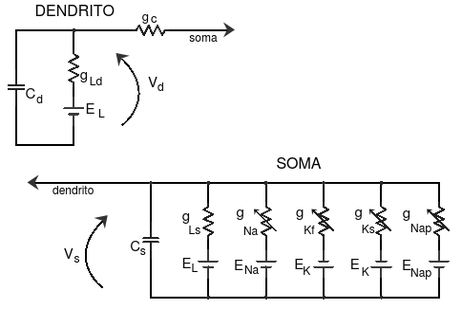
\includegraphics[width=7cm]{../figures/pdf/Circuito}}
  \caption{Circuito elétrico equivalente representando o soma e o dendrito dos modelos de MNs. $E_Na$ e $E_K$ representam os potenciais de equilíbrio dos íons Na+ e K+, respectivamente. $E_L$ representa o potencial de repouso da membrana. As condutâncias $g_Ld$, $g_Ls$, $g_c$, $g_Na$,$g_Kf$, $g_Ks$, $g_Nap$, representam as condutâncias de fuga dendrítica e somática, de acoplamento, de Na+, rápida de K+, lenta de K+ e persistente de Na+, respectivamente. $C_d$ e $C_s$ representam as capacitâncias de membrana dendrítica e somática.}
  \label{fig:fig1}
\end{figure}

Para o axônio, adotou-se um modelo simplificado baseado na detecção de um PA e sua transmissão até a UM com uma dada velocidade de condução. Os valores de velocidade de condução axonal foram baseados em estudos anteriores [5] (Tabela 2). O limiar de detecção do PA foi definido como o instante em que a taxa de variação do potencial de membrana é igual (ou ligeiramente superior) a 10mV/ms [4]. Adotou-se uma distância de 0,60 m entre o MN e a UM.

\paragraph{Modelo de Unidade Muscular}
As UMs foram modeladas como a resposta ao impulso (em tempo discreto) de um sistema de segunda ordem criticamente amortecido. Neste sistema são definidos dois parâmetros: i) a amplitude máxima do abalo muscular e ii) o tempo de contração (intervalo entre o início do abalo e o instante em que se atinge a amplitude máxima). Além disso, adotou-se um mecanismo forçado de saturação (baseado na frequência de disparos de PAs do MN) para as forças tetânicas das UMs. Os parâmetros dos modelos das UMs dos tipos S, FR e FF encontram-se na Tabela 2 e foram baseados em dados experimentais do tríceps sural humano [14].

\begin{table}[h]
 \caption{Parâmetros dos modelos de MN.}
  \centering
  \begin{tabular}{llll}
    \toprule
   % \multicolumn{2}{c}{Part}                   \\
    %\cmidrule(r){1-2}
    Parâmetro     & Tipo S     & Tipo FR     & Tipo FF   \\
    \midrule
    Capacitância específica [F/cm2] & 1 & 1 & 1    \\
    Resistividade citoplasmática [Ohm-cm2] & 70 & 70 & 70 \\
    Comprimento (dendrito) [mm] & 6,15 & 7,45 & 9,35 \\
    Diâmetro (dendrito) [um] & 52 & 73 & 88 \\
    Resistência específica (dendrito) [kOhm-cm2] & 12,55 & 8,83 & 6,50 \\
    Comprimento (soma) [um] & 80 & 85 & 100,25 \\
    Diâmetro (soma) [um] & 80 & 85 & 100,25 \\
    Resistência epecífica (soma) [kOhm-cm2] & 1,10 & 1,0 & 0,80 \\
    Velocidade de condução axonal [m/s] & 45,5 & 48,5 & 51,5 \\
   % Axon     & Output terminal & $\sim$10      \\
    %Soma     & Cell body       & up to $10^6$  \\
    \bottomrule
  \end{tabular}
  \label{tab:table}
\end{table}

% Size ($\mu$m);   $\sim$100

\begin{table}[h]
 \caption{Parâmetros das unidades musculares.}
  \centering
  \begin{tabular}{llll}
    \toprule
   % \multicolumn{2}{c}{Part}                   \\
    %\cmidrule(r){1-2}
    Parâmetro     & Tipo S     & Tipo FR     & Tipo FF   \\
    \midrule
    Amplitude do abalo [N] & 1,70 & 1,90 & 2,15 \\
    Tempo de contração [ms] & 110,0 & 73,5 & 55,0 \\
    Frequência de saturação [Hz] & 20 & 40 & 60 \\
    \bottomrule
  \end{tabular}
  \label{tab:table}
\end{table}

\paragraph{Protocolo de Simulação: Relação força-frequência das unidades motoras}
Todas as simulações foram realizadas utilizando-se o método numérico de integração de Euler com passo fixo de 1 ms. Foram realizados dois protocolos experimentais que serão descritos a seguir. Foram feitas simulações para verificar a relação entrada-saída de cada unidade motora. Para tanto, cada MN do núcleo motor foi estimulado com degraus de corrente com diferentes intensidades, de forma a promover disparos repetitivos de PAs com diferentes frequências. Em cada condição, registrou-se a força gerada pelas unidades motoras a fim de se obter a relação entre a força da UM e a frequência de ativação do MN [15].

\paragraph{Protocolo de simulação: Princípio do tamanho e geração da força muscular}
Neste protocolo, buscou-se verificar a capacidade do modelo em representar as duas estratégias principais do sistema neuromuscular no controle de força: o recrutamento de unidades motoras (recruitment coding) e a modulação de suas frequências de disparos de PA (rate coding) [16]. O núcleo motor foi estimulado por uma corrente com forma de onda triangular simétrica (pico de 22 nA) e duração de 5 segundos. A força total gerada pelo modelo simplificado de músculo foi definida como a soma das forças geradas pelas UMs.